%-------------------------------------------------------------------------------
\section{Modeling Software Dependencies with ASP}
%-------------------------------------------------------------------------------
\label{sec:asp-model}

At a high-level, with the introduction of \clingo, each concretization
combines:
\begin{enumerate}
\item A large number of \emph{facts} characterizing the specific problem being solved
\item A small \emph{logic program} encoding the rules and constraints of the software model
\end{enumerate}
The facts are always generated starting from one or more 
\emph{root specs} that need to be concretized, and they account 
for both the metadata contained in package recipes and the 
current state of \spack{} in terms of configuration and 
installed software.
For instance, a simple directive such as:
\begin{minted}[fontsize=\small, bgcolor=bg]{python}
version('1.2.11', sha256='ah45rstgef...')
\end{minted}
in \texttt{zlib}'s recipe is translated to the following fact:
\begin{minted}[fontsize=\small, bgcolor=bg]{text}
version_declared("zlib", "1.2.11", 0, "package_py").
\end{minted}
in our ASP solve. Similarly, the request to concretize
\begin{minted}[fontsize=\small, bgcolor=bg]{text}
zlib@1.2.11
\end{minted}
generates the following three facts:
\begin{minted}[fontsize=\small, bgcolor=bg]{text}
root("zlib").
node("zlib").
version_satisfies("zlib","1.2.11").
\end{minted}
stating that \texttt{zlib} is a root node and should satisfy
a version requirement.
A typical solve has around $10k-100k$ facts which include
the encoding of dependencies, variants, preferences, etc.

The logic program encodes the software model used by \spack{}
and is solely composed by first-order rules, integrity 
constraints and optimization objectives. 
The declarative nature of ASP makes it easy to enforce 
certain properties on the optimal solution. For instance, 
these three lines ensure that we never have a cyclic dependency
in a DAG:
\begin{minted}[fontsize=\small, bgcolor=bg]{text}
path(A, B) :- depends_on(A, B).
path(A, C) :- path(A, B), depends_on(B, C).
:- path(A, B), path(B, A).
\end{minted}
The first rule establishes the base case: if \texttt{A} depends
on \texttt{B} there is a path from \texttt{A} to \texttt{B}.
The second rule defines paths to transitive dependencies 
with a recursive definition: if there is a path from \texttt{A} 
to \texttt{B} and \texttt{B} depends on \texttt{C}, there is
a path from \texttt{A} to \texttt{C}. The final line is an 
\emph{integrity constraints} stating that paths from \texttt{A} 
to \texttt{B} and paths from \texttt{B} to \texttt{A} cannot 
occur at the same time in a valid solution.

To give a rough idea of the compactness and expressiveness of 
the ASP encoding, the entire logic program for the software 
model described in Section~\ref{sec:software-model} is around 
$500$ lines of code. The concretization process is straightforward
to follow conceptually within \spack:
\begin{enumerate}
\item Facts are generated for the current concretization \footnotemark
\item The logic program and the facts are sent to the solver
\item The concretized DAG is rebuilt from the \emph{optimal} result
\end{enumerate}
\footnotetext{It's worth stressing that the logic program changes only
when the underlying software model changes, as opposed 
to the generated facts that are different whenever the root
spec to be concretized or \spack's configuration changes.}
The word ``optimal'' is emphasized since, while rules and integrity 
constraints fully determine if a solution is valid, we need 
optimization targets to select one of the many possible solutions
in a way that fits user's expectations.

A good example to illustrate this point is target selection for DAG nodes.
In \spack{} each node being built has a target microarchitecture associated with it, and we want to use the best target possible while respecting the constraints coming from the compiler (some compilers don't support generating code for some targets) and from the configuration. 
Previously this required some complicated logic mixed with the rest of the solve.
The introduction of \clingo{} simplified the problem definition by a great amount. A cardinality constraint is used to express that each node must have one and only one target:
\begin{minted}[fontsize=\small, bgcolor=bg]{text}
1 { node_target(Package, Target) : 
    target(Target) } 1 :- node(Package).
\end{minted}
A rule ensures that the user's choice to set the target to a specific value is respected:
\begin{minted}[fontsize=\small, bgcolor=bg]{text}
node_target(P, T) :- node(P), node_target_set(P, T).
\end{minted}
An integrity constraints prevents to choose a target not supported by the current compiler:
\begin{minted}[fontsize=\small, bgcolor=bg]{text}
:- node_target(P, T),
   not compiler_supports_target(C, V, T),
   node_compiler(P, C),
   node_compiler_version(P, C, V).
\end{minted}
These three statements fully describe the characteristics of a valid solution. To pick the \emph{optimal} solution we also \emph{weight} the possible targets
(the lower the weight, the best the target) and optimize over the sum of target weights:
\begin{minted}[fontsize=\small, bgcolor=bg]{text}
node_target_weight(P, W) :- 
  node(P), node_target(P, T), target_weight(T, W).
#minimize { W@5,P : node_target_weight(P, W) }.
\end{minted}

\subsection{Generalized Condition Handling}
\label{subsec:generalizedcond}
A peculiar feature of \spack, as a package manager, is that it doesn't only optimize for versions but for many other aspects of the build as well e.g. which compiler to use, which microarchitecture to target, etc. 
The DSL used for package recipes reflects this complexity by having multiple directives to declare different properties or constraints for each software, as seen in Section~\ref{sec:software-model}. 

One interesting abstraction, that we observed while coding the ASP logic program, is that each of these directives can be seen as a way to impose additional constraints on the solution, conditional on other constraints 
being met. For instance, the following directive in a package:
\begin{minted}[fontsize=\small, bgcolor=bg]{python}
depends_on('hdf5+mpi', when='+mpi')
\end{minted}
means that, if the spec has the \texttt{mpi} variant turned on, then it depends on \texttt{hdf5+mpi}. Similarly:
\begin{minted}[fontsize=\small, bgcolor=bg]{python}
provides('lapack', when='@12.0:')
\end{minted}
means that a package provides the \texttt{LAPACK} API if its version is $12.0$ or greater.
This property allowed to encode all the directives as \emph{generalized conditions}, where most of the sematics is encoded abstractly in a few lines of the logic program.

Getting back to a simple example, the snippet below:
\begin{minted}[fontsize=\small, bgcolor=bg]{python}
class H5utils(AutotoolsPackage):
    depends_on('png@1.6.0:', when='+png')
\end{minted}
is translated to the following facts:
\begin{minted}[fontsize=\scriptsize, bgcolor=bg]{text}
condition(153).
condition_requirement(153, "node", "h5utils").
condition_requirement(153, "variant_value", "h5utils", "png", "true").
imposed_constraint(153, "version_satisfies", "libpng", "1.6.0:").
dependency_condition(153, "h5utils", "libpng").
\end{minted}
when setting up the problem to be solved by \clingo. The important points to note are that:
\begin{itemize}
\item Each directive is associated with a unique global ID.
\item Constraints are either ``requirement'' or ``imposed''. 
\item Different type of conditions have different semantics\footnotemark
\end{itemize}
\footnotetext{For instance, the \texttt{dependency\_condition} fact is present only for \texttt{depends\_on} directives and activates logic that is specific to dependencies.}
The code to trigger and impose general conditions in the logic program is surprisingly simple to read. ASP conditional rules allow us to effectively build new rules from input facts:
\begin{minted}[fontsize=\small, bgcolor=bg]{text}
condition_holds(ID) :-
condition(ID);
attr(N, A1): condition_requirement(ID, N, A1);
attr(N, A1, A2): condition_requirement(ID, N, A1, A2);
...
\end{minted}
based on their \emph{arity}. Other rules, similar to:
\begin{minted}[fontsize=\small, bgcolor=bg]{text}
attr(N, A1) :- 
  condition_holds(ID), imposed_constraint(ID, N, A1).
\end{minted}
enforce the imposed constraints when a condition holds.

\subsection{Usability Improvements due to \clingo}
Before the adoption of \clingo, concretization in \spack{} was performed relying on a greedy algorithm with limited backtracking capabilities. This algorithm ensured only that solutions found are valid and conforming to user's request, but it might have failed to find one of those valid solutions if backtracking was necessary to reach that result. Said otherwise, the old algorithm was subject to outputing many \emph{false negatives} \textemdash{} cases where \spack{} would error even though a valid solution exists.

A workaround for this limitation consisted in overconstraining problematic specs, so to make backtracking unnecessary. The drawback was an increased need for boilerplate code, which became particularly evident in large production environments and complex scientific software. With the adoption of \clingo{} overspecification is not needed anymore and \emph{false negatives} have been effectively eliminated from concretization.

\subsubsection{Conditional Dependencies}
A prominent example of this behavior is with packages having dependencies conditional to a variant being set to a non-default value. Let's take for instance \texttt{hpctoolkit}, which has the following directives:
\begin{minted}[fontsize=\small, bgcolor=bg]{python}
class Hpctoolkit(AutotoolsPackage):
    variant('mpi', default=False, description='...')
    depends_on('mpi', when='+mpi')
\end{minted}
Trying to use the old algorithm to concretize \texttt{hpctoolkit \^{}mpich} fails like shown next:
\begin{minted}[fontsize=\footnotesize, bgcolor=bg]{console}
% spack spec hpctoolkit ^mpich
Input spec
--------------------------------
hpctoolkit
    ^mpich

Concretized
--------------------------------
==> Error: Package hpctoolkit does not depend on mpich
\end{minted}
since the greedy algorithm would set variant values before descending to dependencies. Since no value is specified for the \texttt{mpi} variant, the value chosen is \texttt{false} (the variant default) which leads to \texttt{hpctoolkit} having no dependency on \texttt{mpi}. The workaround required users to write the redundant spec \texttt{hpctoolkit+mpi \^{}mpich} to be able to concretize succesfully. With \clingo{} the overspecification is not needed anymore and the value of the \texttt{mpi} variant is correctly deduced from the user's request to have \texttt{mpich} in the graph, as shown
in Figure~\ref{fig:hpctoolkit}.

% FIXME: Figure is too small, what should we do about that? Remove it? Show only part?
\begin{figure}[h]
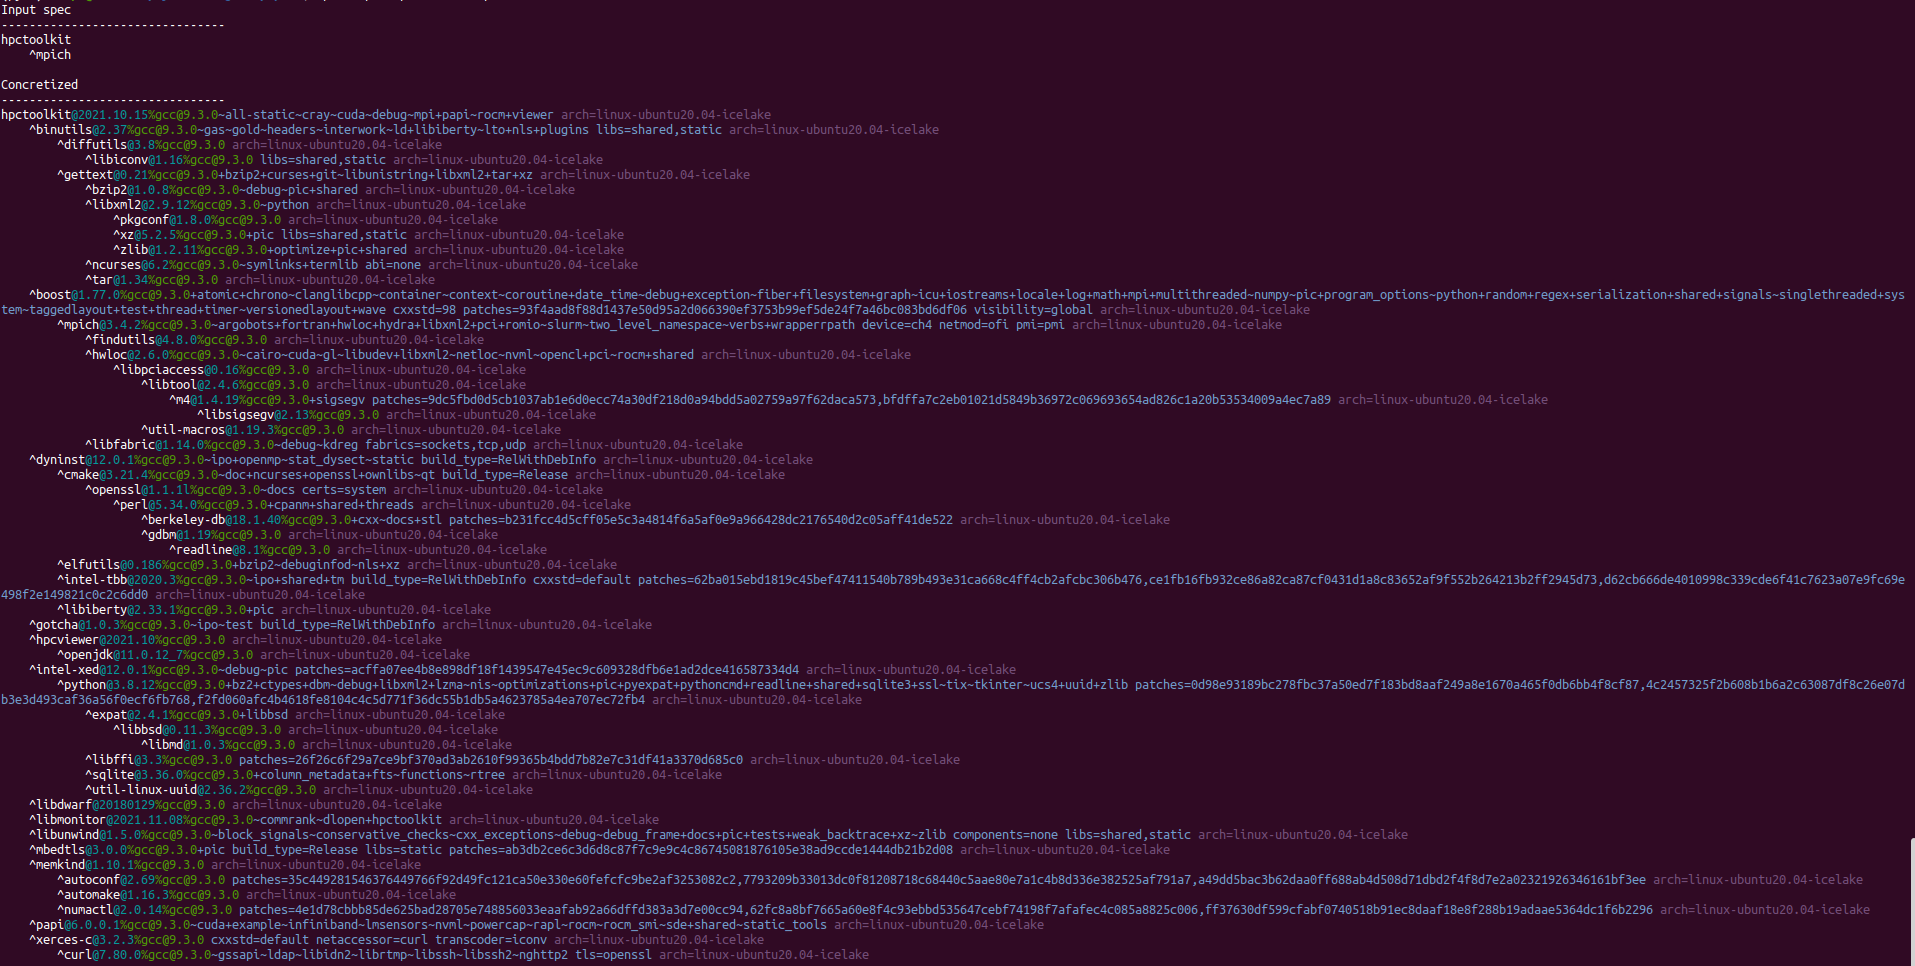
\includegraphics[width=\columnwidth]{figures/hpctoolkit_concretized.png}
\caption{\texttt{hpctoolkit \^{}mpich} as concretized on an Ubuntu 20.04 OS using system compilers}
\label{fig:hpctoolkit}
\end{figure}

\subsubsection{Conflicts in Packages}
Before using \clingo{} conflicts in packages were only used to \emph{validate} a solution computed by the greedy-algorithm. If the solution matched any conflict, \spack{} would have errored and hinted the user on how to overconstrain the initial spec to help concretization. With clingo instead conflicts are fully taken into account during the solve\footnotemark{} and \spack{} can succesfully find solutions without asking the user to be more specific.
\footnotetext{With \clingo{} conflicts are treated as shown in Section~\ref{subsec:generalizedcond} and, by imposing \emph{integrity constraints} on the problem, they effectively prevent portions of the search space from being explored}

\subsubsection{Specialization on Providers of Virtual Packages}
Using \clingo{} also enabled more complex use cases e.g. imposing constraints on specific virtual package providers. A simple example of that is given by the \texttt{berkeleygw} package, which has the following directives:
\begin{minted}[fontsize=\small, bgcolor=bg]{python}
class Berkeleygw(MakefilePackage):
    variant('openmp', default=True)
    depends_on('lapack')
    depends_on('openblas threads=openmp', 
               when='+openmp ^openblas')
\end{minted}
The last directive forces \texttt{openblas} to have \texttt{openmp} support if \texttt{berkeleygw} has \texttt{openmp} support and \texttt{openblas} has been chosen as a provider for the mandatory \texttt{lapack} virtual dependency. Conditional constraints of that complexity could not be expressed before, due to the limitations of the previous greedy algorithm.
